\chapter[Simulação e Resultados]{Simulação e Resultados}

%\section{asdf}
A simulação foi realizada no Cadence usando a tecnologia 0.18 UMC. Para observar a ativação de todas as faixas de frequência fornecidas pelo circuito, foram ajustadas 3 fontes com atraso de início para ativar as entradas no integrador. Ao fazer a simulação transiente as faixas de frequência obtidas foram:
%[V]	[T C°]	[CORNER]   [ADJ1] & [ADJ2]   [ADJ3]
%1.2	  36	 typ	   101.4 &  1.092K &  10.722K
%2.5	  36 	 typ 	   997.7 &  9.717K &  98.325K

\begin{itemize}
\item 101,4Hz	 \----	997,7Hz
\item 1,092KHz \----	9,717KHz
\item 10,722KHz \----	98,325KHz
\end{itemize}

A potência máxima consumida é obtida quando o VFC fornece a maior frequência possível. Ao fornecer uma tensão $V_{in}$ de 2,5V e o resto do circuito com tensão de alimentação $V_{DD}$ de 1,2V a máxima potência média calculada foi de $956,2n$W.


\begin{figure}[htb]
	\centering
	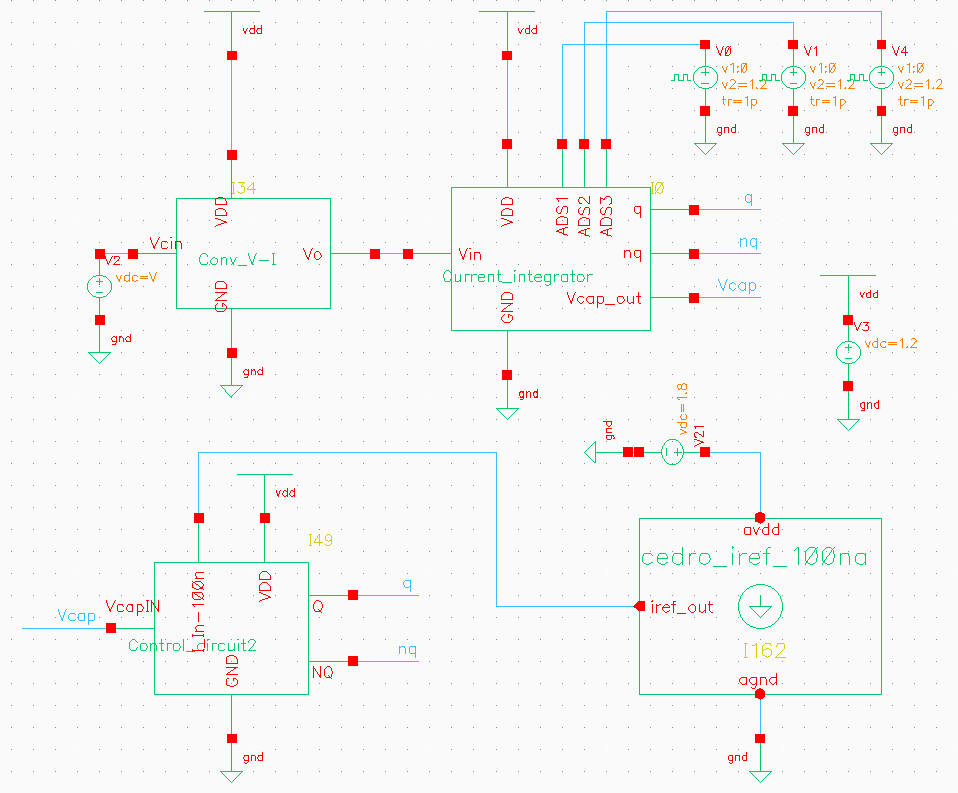
\includegraphics[width=0.9\textwidth]{figuras/imgs_jv/top.png}
	\caption{ Esquemático de topo com integração de todos os sub-circuitos do projeto }
	\label{fig16}
\end{figure}

\section{Conversor tensão corrente}

A relação entre a tensão $V_{in}$ e a corrente de saída do VIC está na Fig. \ref{fig17}. Observa-se no gráfico que os limites da faixa de correntes mínimas e máximas são:
\begin{itemize}
\item $1,2$V	 \----	$68,2n$A
\item $2,5$V \----	$703,7n$A
\end{itemize}




As correntes espelhadas no integrador seguem o comportamento desse conversor, portanto a linearidade de ambos são iguais. Por conta disso um VIC mal feito acarretaria erros acumulados, como pouca linearidade, faixa de frequência e consumo de potência, que dificultariam o funcionamento esperado dos outros circuitos.


\begin{figure}[htb]
	\centering
	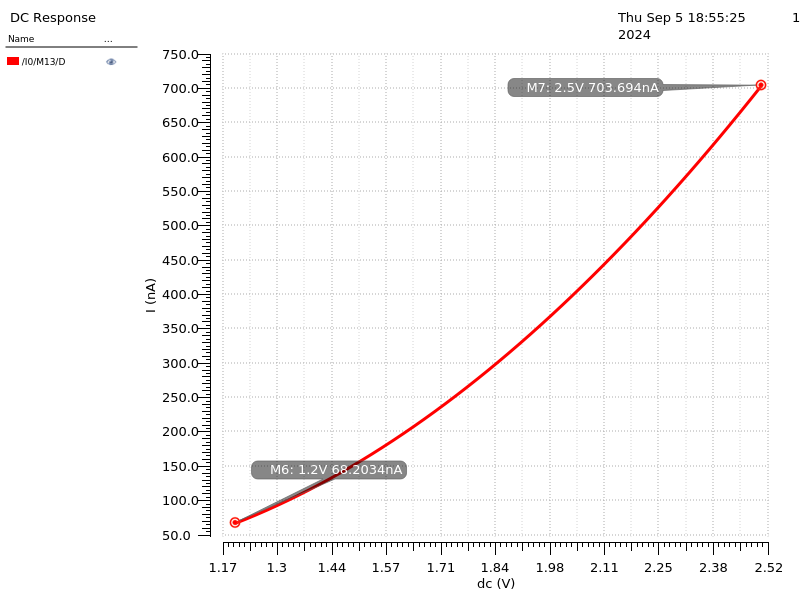
\includegraphics[width=0.9\textwidth]{figuras/imgs_jv/sim_VIC2.png}
	\caption{ Simulação da corrente de referência espelhada na Saída do VIC }
	\label{fig17}
\end{figure}


\section{Latch SR}

Na Fig. \ref{fig18} está a simulação do Latch SR, que foi implementado no circuito de controle. Nela foi testado o comportamento dele para comparar com a sua tabela lógica da Fig. \ref{fig14}.  Em vermelho está o sinal de $R$, em verde $S$, roza $q$ e em ciano $nq$.

\begin{figure}[htb]
	\centering
	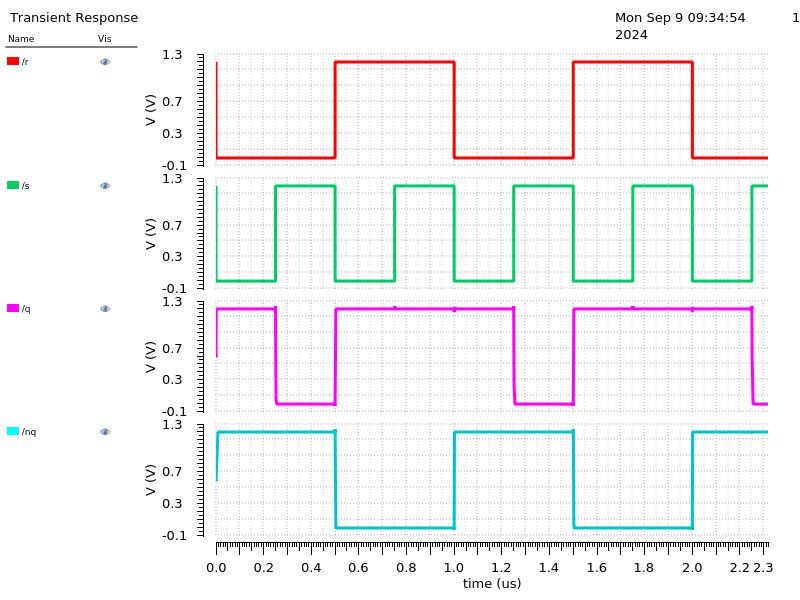
\includegraphics[width=0.9\textwidth]{figuras/imgs_jv/sim_lach.jpg}
	\caption{Simulação do Latch SR no Cadence }
	\label{fig18}
\end{figure}


\section{Amplificador operacional}

O AmpOp usado para a elaboração do circuito de controle foi simulado de forma isolada para análise de desempenho. Na Fig. \ref{fig19} estão exibidos em azul o ganho em decibéis e a fase em vermelho, ambos analisados com o variar da frequência.

\begin{figure}[htb]
	\centering
	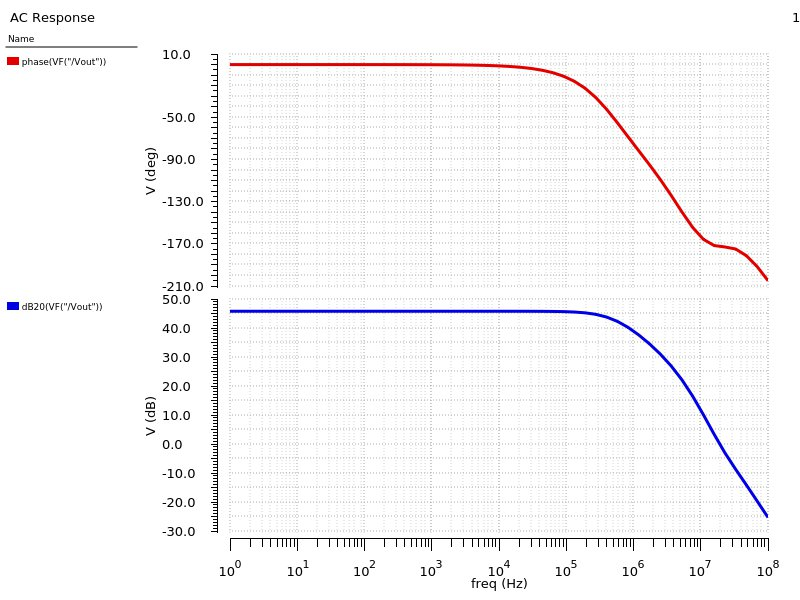
\includegraphics[width=0.9\textwidth]{figuras/imgs_jv/sim_ampop.jpg}
	\caption{ Simulação no Cadence do modelo de AmpOp usado no circuito de controle }
	\label{fig19}
\end{figure}



\section{Circuito de Controle}

Na Fig. \ref{fig24} está os sinais observados no circuito de controle. Nota-se o acionamento dos sinais $Q$(verde), e $NQ$(vermelho), no Latch com a queda abrupta nos AmpOps nos sinais $R$(rosa), e $S$(laranja). O sinal de resposta do comparador do sistema de controle, ao perceber que $V_{cap}$(azul), atingiu $V_H$, cai e aciona no Latch a rotina de descarga do capacitor. Inversamente ao perceber que $V_{cap}$ ficou menor que $V_L$ o sinal $S$ cai e o Latch aciona a rotina de carga.

A tensão $V_{cap}$ é observada na onda triangular em azul e a onda quadrada é o sinal em frequência do VFC e saída $Q$ do Latch.
Vale salientar que na Fig. \ref{fig23} há marcações nos pontos máximos e mínimos do sinal do capacitor. Isso porque ao aumentar a frequência do sinal a resposta dos AmpOps do circuito de controle fica mais lenta, então os limites da tensão $V_{cap}$ se alargam, abrangendo uma faixa de tensão maior. A variação varia dependendo se o limite é superior ou inferior, mas nessa frequência máxima a média do desvio é cerca de 21$m$V.  

\begin{figure}[htb]
	\centering
	 \begin{subfigure}[b]{0.49\textwidth}
	  \centering
	  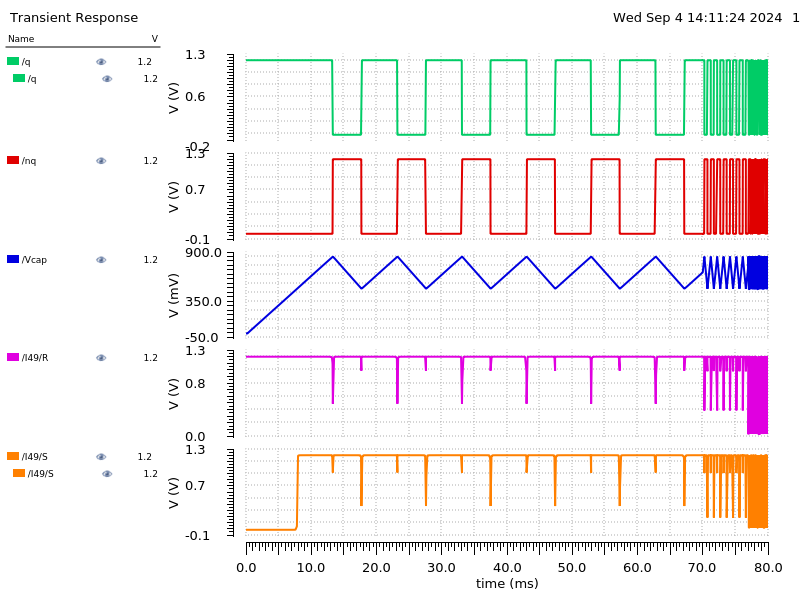
\includegraphics[width=\textwidth]{figuras/imgs_jv/waves_1-2_parte1.png}       
    \caption{Gráfico da simulação com $V_{in}=1,2V$}
    \label{fig20}
   \end{subfigure}
	 \begin{subfigure}[b]{0.49\textwidth}
	  \centering
	  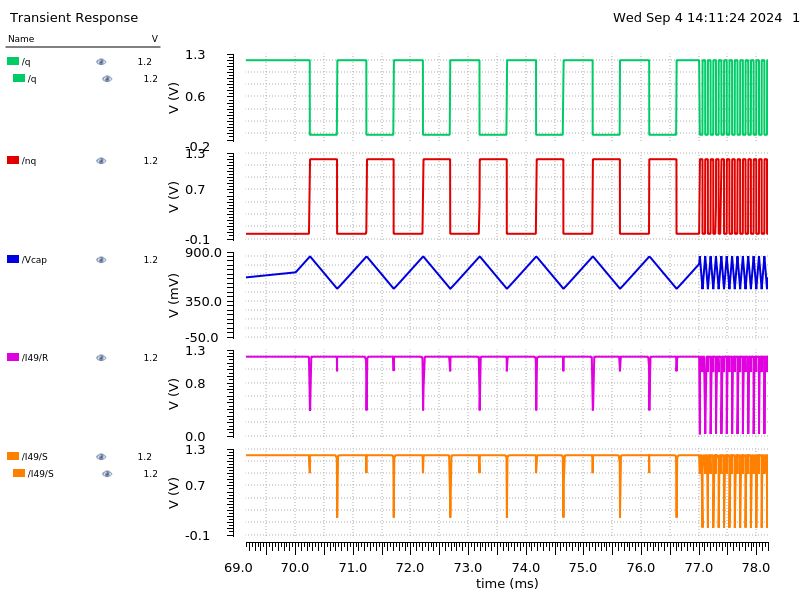
\includegraphics[width=\textwidth]{figuras/imgs_jv/waves_1-2_parte2.png}       
    \caption{Gráfico da simulação com $V_{in}=1,2V$ com zoom nos sinais de maior frequência}
    \label{fig21}
   \end{subfigure}
\hfill 
	 \begin{subfigure}[b]{0.49\textwidth}
	  \centering
	  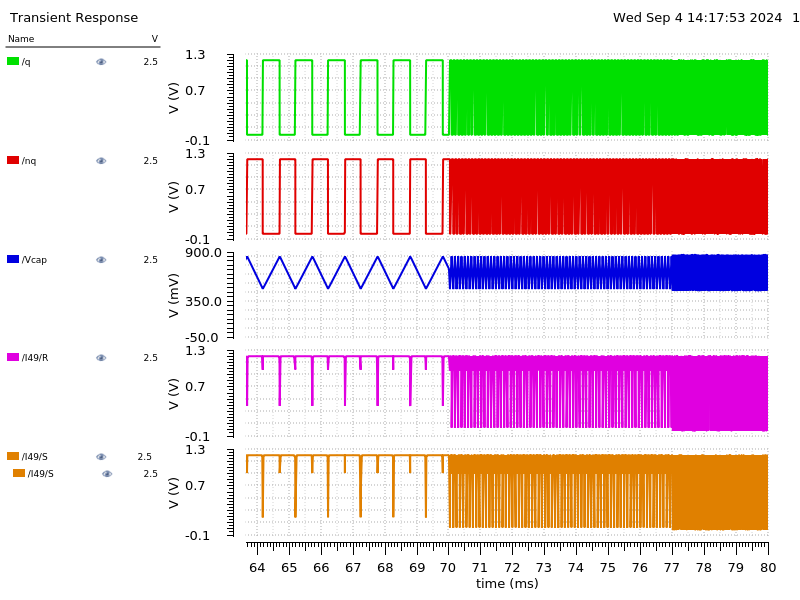
\includegraphics[width=\textwidth]{figuras/imgs_jv/waves_2-5_parte1.png}       
    \caption{Gráfico da simulação com $V_{in}=2,5V$}
    \label{fig22}
   \end{subfigure}
	 \begin{subfigure}[b]{0.49\textwidth}
	  \centering
	  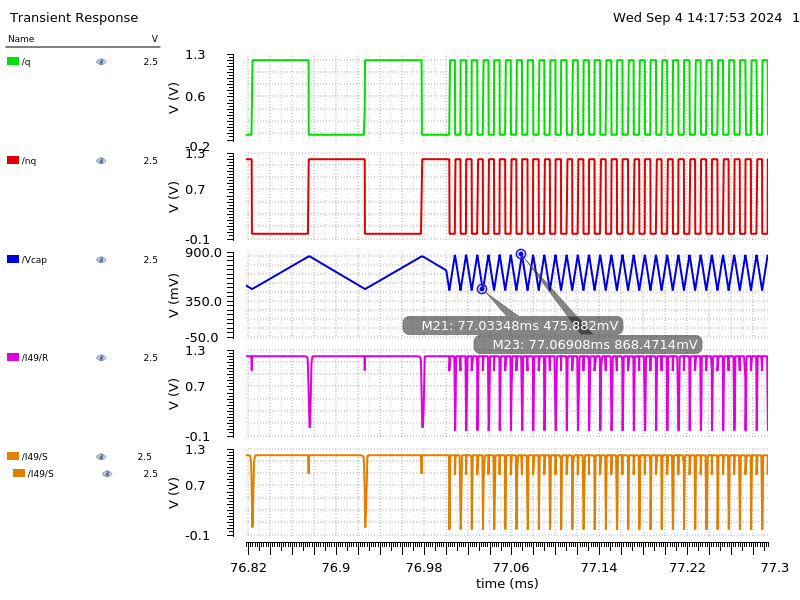
\includegraphics[width=\textwidth]{figuras/imgs_jv/waves_2-5_parte2.png}       
    \caption{Gráfico da simulação com $V_{in}=2,5V$ com zoom nos sinais de maior frequência}
    \label{fig23}
   \end{subfigure}
	\caption{Sinais observados no Circuito de Controle }
	\label{fig24}
\end{figure}



